\section{Results and Discussion}
\label{sec:results}

The environmental setup and a description of the methodology followed for these tests can be found in \cref{sec:environment,sec:methodology}.

The speedups achieved for each test performed on SeARCH Groups 101 and Hex are presented in \cref{fig:speedup}. Regarding the total execution, the MPI version achieves the best values without the Intel\textregistered Hyper-Threading Technology in the Group 101, and with it in Group Hex. Moreover, if one ignores the preparation phase (where the files are loaded and the mesh is partitioned), Intel\textregistered Hyper-Threading Technology allows for a linear speedup from the 24 processes test to the 48 processes test in Group Hex. For the bigger tests (48 and 96 processes in Groups 101 and Hex, respectively), when the number of processes exceeds the available hardware threads the results are worse (yet, in Group Hex this test is still better than the sequential version, which is not the case in Group 101). This is most probably explained by the process scheduling, which greatly affects communication by retaining in the queue one of the two processes communicating. Yet this was not further investigated.

\begin{figure}
	\begin{center}
		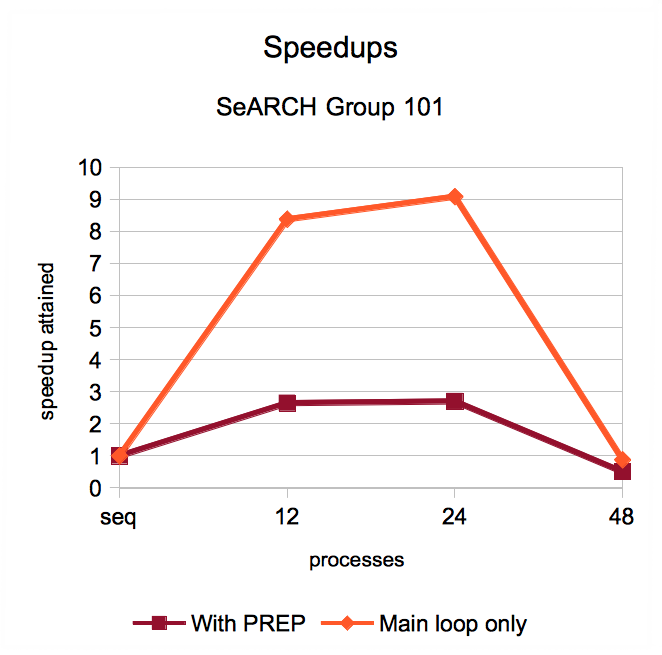
\includegraphics[width=\columnwidth]{report.may/images/speedup101.png}
		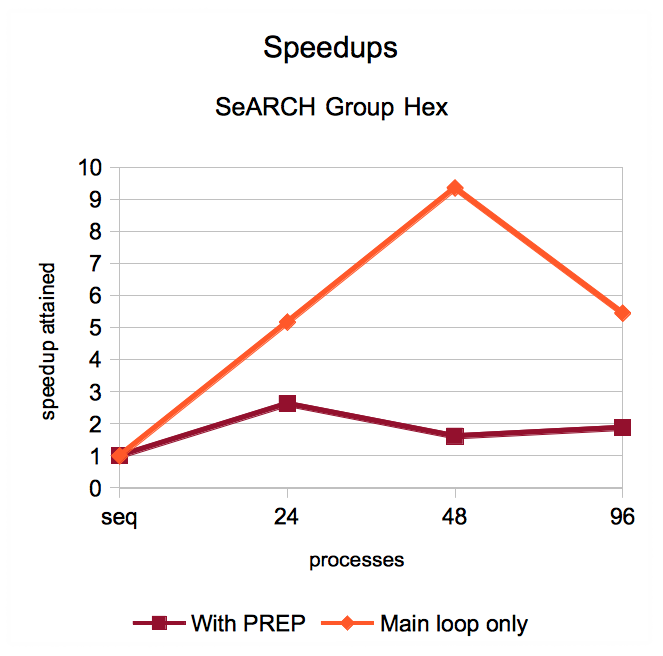
\includegraphics[width=\columnwidth]{report.may/images/speeduphex.png}
	\end{center}
	\caption[Speedups]{Speedups achieved for different numbers of processes on SeARCH Groups 101 and Hex.}
	\label{fig:speedup}
\end{figure}

Analyzing the execution times in \cref{fig:exectime}, one can easily spot the bottlenecks in each test (note the vertical axis, the execution time for the worst case in Group Hex is near the time for the best case in Group 101). For both groups, the sequential version presents the same picture: the update function takes most of the time due to the (already known from previous work) locality problems. For the MPI versions, the bottleneck of the entire execution is obviously the partitioning step, but since it is executed only once, its importance is diminished if the number of iterations is increased. Considering only the main loop, the communication tramples the other core functions, increasing when the number of processes is decreased (larger partitions mean that each inter-node communication holds more data) or increased beyond the hardware parallelism (as explained before, process scheduling hurts intra-node communication).

\begin{figure}
	\begin{center}
		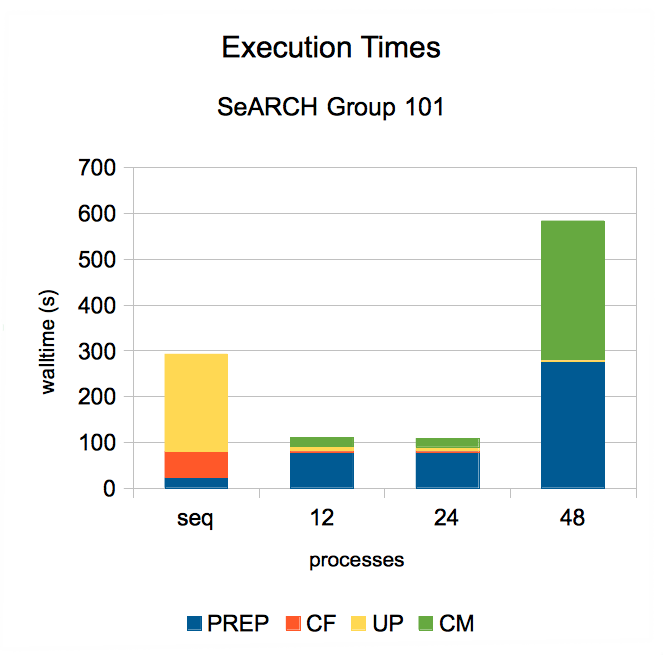
\includegraphics[width=\columnwidth]{report.may/images/exectime101.png}
		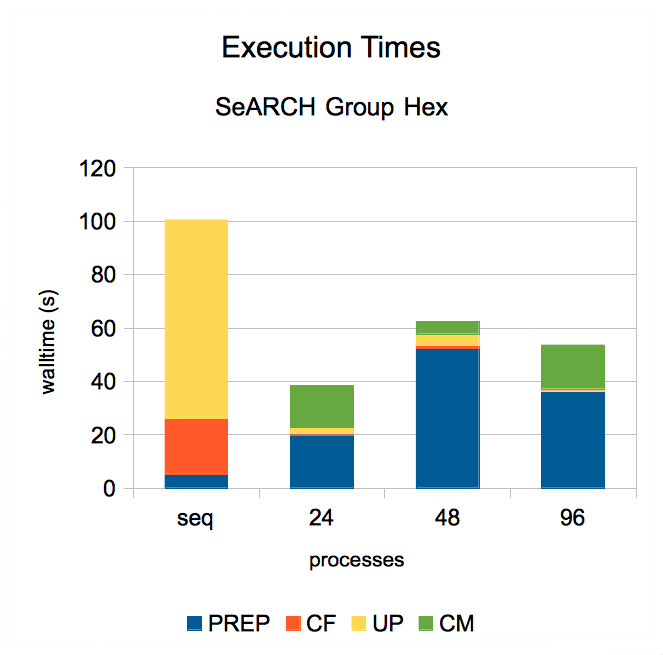
\includegraphics[width=\columnwidth]{report.may/images/exectimehex.png}
	\end{center}
	\caption[Execution times]{Execution times of the tests performed on SeARCH Groups 101 and Hex.}
	\label{fig:exectime}
\end{figure}

\Cref{fig:load1,fig:load2} show the distribution of work in a more obvious way. To note that the parallelism introduced reduces the \texttt{update} function from around 70\% to below 10\% (1\% for the bigger tests). Also noticeable is how the the preparation step and the communication domination change for different numbers of processes in the two node groups. In both groups, the introduction of Intel\textregistered Hyper-Threading Technology causes the partitioning process (memory-bound and mainly sequential, but with some parallelism) to be extended due to thread competition for resources. Then again, the increased number of processes causes partitions to be smaller, which reflects in a speedup in the communication step (very slight decrease in Group 101 but decreases to a fifth in Group Hex). Despite this, when the number of processes increases beyond the hardware available, as explained above the process scheduling will cause communication to take longer. In both Groups, this reflects in a very fast execution of \texttt{update} and \texttt{compute\_flux}, but 99\% of the whole program is spent in the preparation step and with communication.

\begin{figure*}[!p]
	\begin{center}
		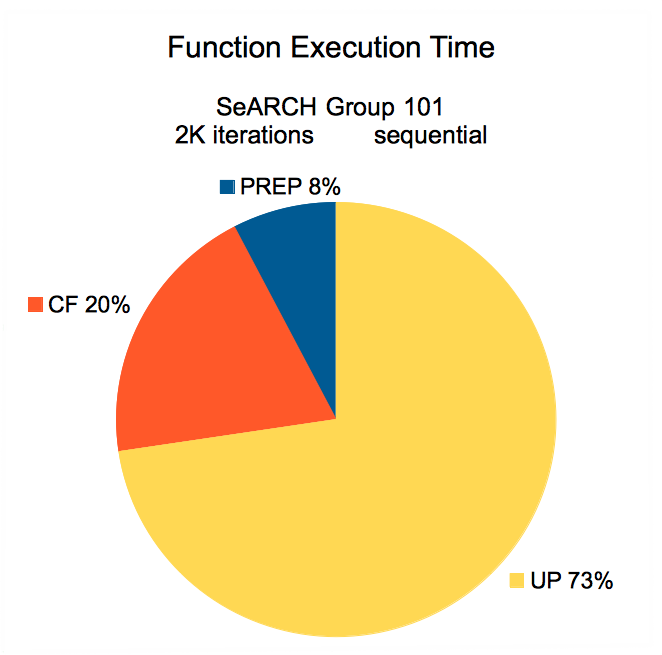
\includegraphics[width=\columnwidth]{report.may/images/loadseq101.png}
		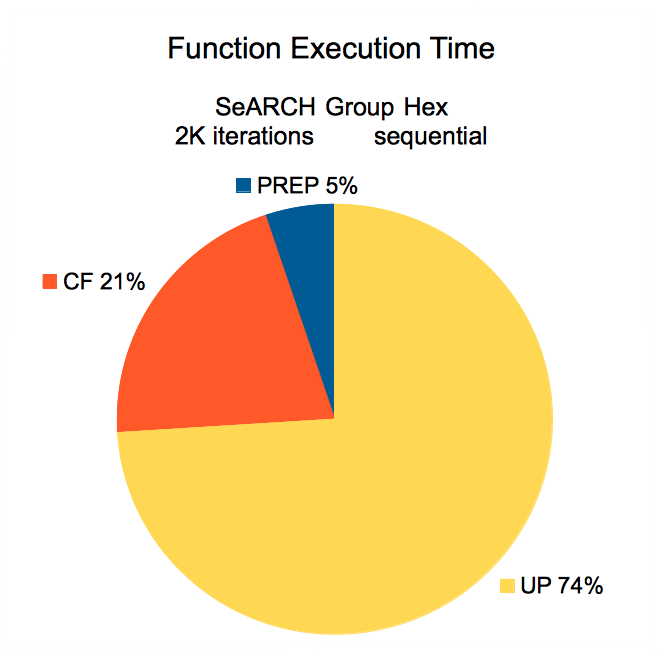
\includegraphics[width=\columnwidth]{report.may/images/loadseqhex.png}
		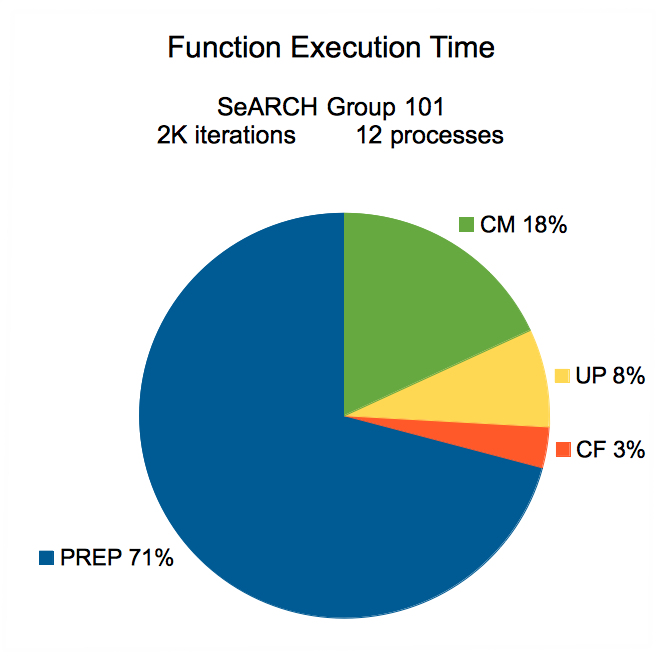
\includegraphics[width=\columnwidth]{report.may/images/load12101.png}
		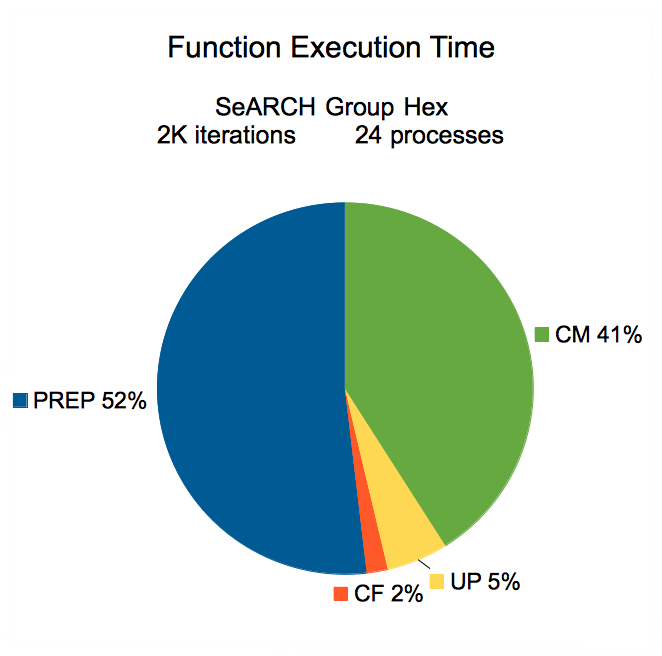
\includegraphics[width=\columnwidth]{report.may/images/load24hex.png}
	\end{center}
	\caption[Work loads]{Median work load of each part of the program in an execution, for the sequential version and the MPI version using half of the available hardware threads on SeARCH Groups 101 and Hex.}
	\label{fig:load1}
\end{figure*}

\begin{figure*}[!p]
	\begin{center}
		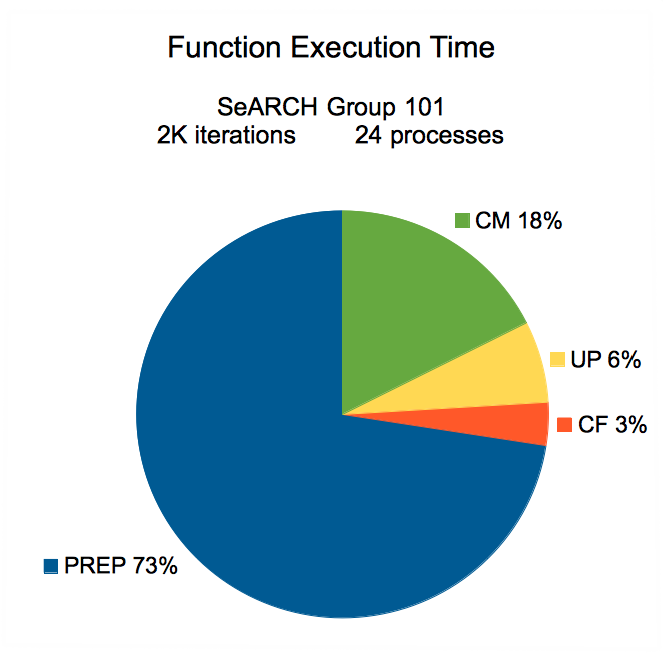
\includegraphics[width=\columnwidth]{report.may/images/load24101.png}
		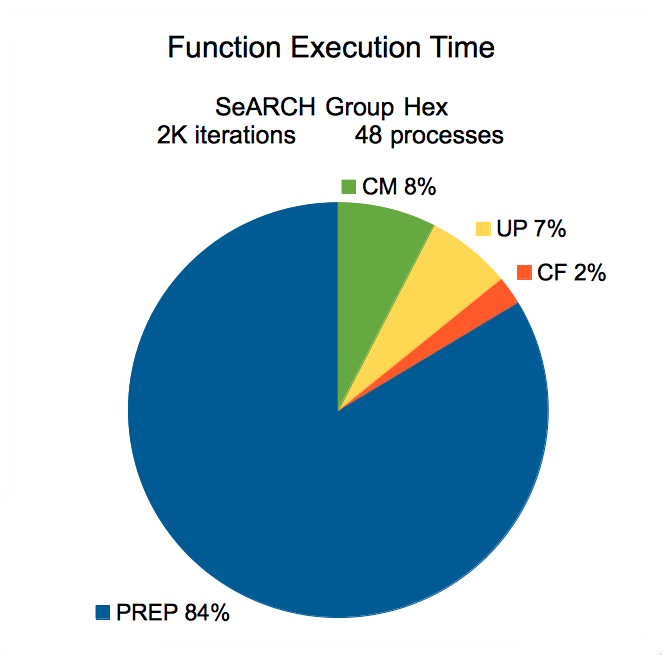
\includegraphics[width=\columnwidth]{report.may/images/load48hex.png}
		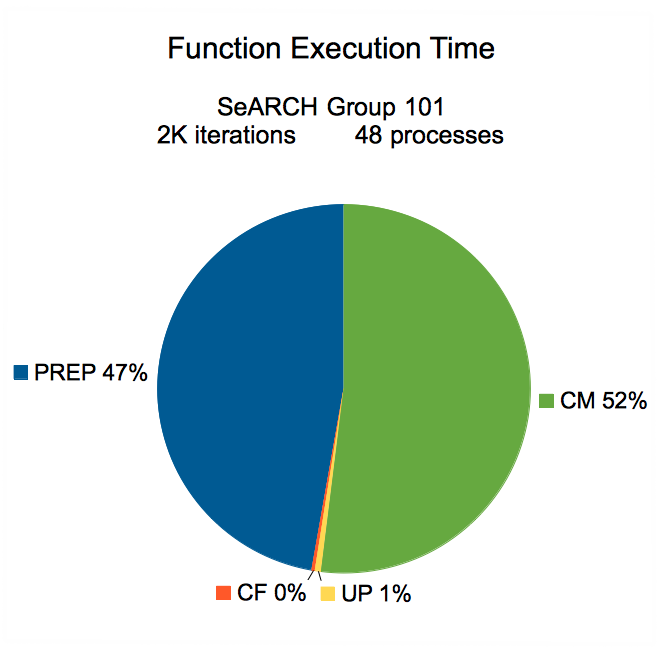
\includegraphics[width=\columnwidth]{report.may/images/load48101.png}
		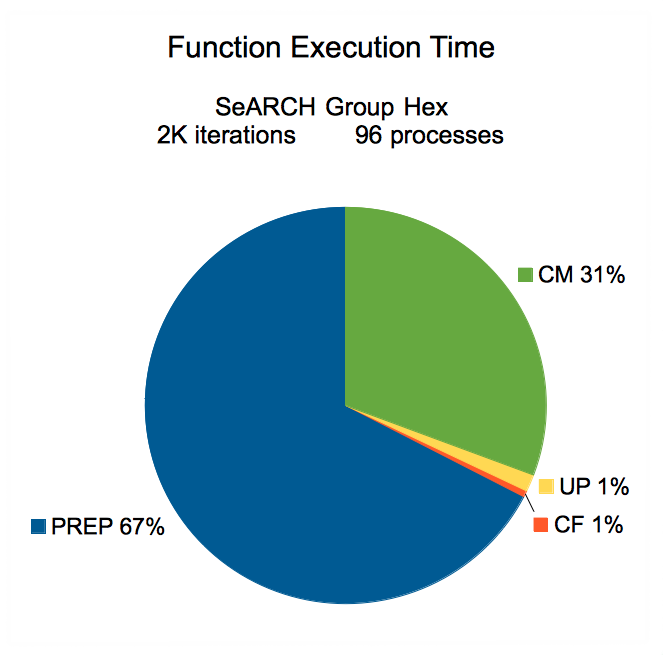
\includegraphics[width=\columnwidth]{report.may/images/load96hex.png}
	\end{center}
	\caption[Work loads]{Median work load of each part of the program in an execution, for the MPI version issuing processes in the exact number and the double of the available hardware threads on SeARCH Groups 101 and Hex.}
	\label{fig:load2}
\end{figure*}
